\documentclass[a4paper,11pt,openright,oneside]{report}
\usepackage[utf8]{inputenc}
\usepackage[T1]{fontenc}
\usepackage[portuguese]{babel}
\usepackage{graphicx}
\usepackage[backend=biber, style=ieee]{biblatex}
\usepackage{csquotes}
\usepackage{blindtext}
\usepackage[printonlyused]{acronym}
\usepackage{hyperref}
\usepackage{indentfirst}
\usepackage[titletoc,title]{appendix}
\usepackage{mathtools}
\usepackage{amsmath,amsthm,amsfonts,amssymb}
\usepackage{caption}
\usepackage{subcaption}
\newcommand{\RNum}[1]{\uppercase\expandafter{\romannumeral #1\relax}}

\bibliography{report.bib}

\begin{document}

\begin{titlepage}
\begin{center}

{\vspace*{50mm}\textsc{\Huge\textbf{Bloom-filter + Locality-Sensitive Hashing}\\ \small{Métodos Probabilísticos para Engenharia Informática}}}\\[2cm]
{\textsc{\small\textbf{Universidade de Aveiro}}}\\[0.5cm]
{\small Pedro Martins 76551\\Ricardo Jesus 76613}\\[0.5cm]
{\small	17 de Dezembro de 2015}\\

\begin{figure}[b]
\center
\graphicspath{}

\includegraphics[height=2cm]{ua.pdf}
\end{figure}

\end{center}

\end{titlepage}

\title{\textbf{Bloom-filter + Locality-Sensitive Hashing}\\[1cm]\textsc{\small {Departamento de Electrónica, Telecomunicações e Informática} \\ \large {UNIVERSIDADE DE AVEIRO}}}
\author{Pedro Martins 76551, pbmartins@ua.pt\\Ricardo Jesus 76613, ricardojesus@ua.pt}
\date{17 de Dezembro de 2015}

\maketitle

\pagenumbering{roman}

\begin{abstract}

ABSTRACT

\end{abstract}

\tableofcontents
%\listoftables
\listoffigures

\clearpage
\pagenumbering{arabic}

\chapter{Introdução}
\label{chap.introdução}

Na área da informática, é, por exemplo, muitas vezes necessário saber se algo pertence a um certo conjunto de forma eficiente. A solução mais óbvia seria percorrer todo o conjunto e comparar, um a um, todos os elementos até encontrar aquele de que se andava inicialmente à procura. No entanto, este método é deveras ineficiente, principalmente se se estiver a trabalhar com conjuntos com milhões ou mais elementos. É aqui que surgem estruturas como \textit{Bloom-filters}. 

\textit{Bloom-filters} usam geralmente várias funções de dispersão (ou \textit{hashing}) para determinar a pertença de um dado elemento num conjunto (\textit{set}). São muito utilizados em grandes conjuntos de dados e em diversas aplicações, como corretores ortográficos de computadores, \textit{smartphones}, etc., análise textual, entre outras. Contudo, e sendo uma estrutura probabilística, acarreta um erro associado.

Outra técnica bastante relevante em situações onde é ``impossível'' guardar e trabalhar enormes conjuntos de dados é o de \textit{MinHash}. Muitas vezes a par com este aparece também o método de \textit{Locality-sensitive hashing (LSH)}, com aplicações usuais em \textit{clustering} de informação e procura de vizinhos próximos a um dado elemento (\textit{nearest neighbor search}).

Neste trabalho, foi desenvolvido em MATLAB um \textit{Bloom-filter}, um \textit{MEX file} fazendo de interface para uma função de \textit{hashing} escrita em C++ e ainda um módulo com capacidade de \textit{nearest neighbor search} utilizando \textit{MinHash} para gerar uma representação de diferentes documentos a serem tratados.

\chapter{Bloom-filter}
\label{chap.bloom}

\textit{Bloom-filters} são estruturas de dados probabilísticas que utilizam uma ou várias funções de \textit{hashing} para determinar a pertença de um dado elemento num \textit{set}. Internamente, habitualmente utilizam um vector de \textit{bits}.

Assumindo funções de \textit{hashing} eficiêntes, mesmo que se opere sobre um conjunto com milhões ou milhares de milhões de elementos, determinar a presença ou não presença nesse conjunto será sempre um processo significativamente mais rápido que caso se iterasse sobre todo o \textit{set}, elemento a elemento, à procura daquele em questão. Este processo depende do número e da qualidade das funções de \textit{hashing} utilizadas.

Como estrutura probabilística que é, tem um erro associado. No entanto este erro manifesta-se apenas em falsos positivos, i.e., se um \textit{Bloom-filter} indica que um elemento pertence a um conjunto, então \underline{provavelmente} ele pertence mesmo. Por outro lado, se um \textit{Bloom-filter} indica que um elemento não pertence a um conjunto, então \underline{definitivamente} ele não pertence. Tendo isto em mente, habitualmente os \textit{Bloom-filters} são dimensionados para um erro máximo admissível e para um determinado número de elementos que se tencione adicionar ao filtro.

Este erro depende do número de \textit{buckets} no vector interno e do número de funções de \textit{hashing} a utilizar. Estas funções devem ser descorrelacionadas entre si e em número variável (para cada conjunto de parâmetros para os quais o filtro é dimensionado). Uma solução para o número variável de funções que se deve considerar é, em vez de se utilizarem $k$ funções diferentes, utilizar-se uma família de funções que garanta $k$ funções descorrelacionadas.

Neste trabalho utilizou-se a família de funções de dispersão denominada \textit{FarmHash}, desenvolvida pela Google, em que um dos argumentos, a \texttt{seed}, permite especificar cada uma das funções da família. A sua implementação é disponibilizada em C++ pela empresa que a desenvolveu (Google), e portanto de forma a poder ser utilizada ao longo do projeto foi escrito um ficheiro \textit{MEX} que permite a interface entre código MATLAB e a função. Caso seja necessário, o ficheiro pode ser compilado executando (no directório onde os ficheiros \textit{.h} e \textit{.cpp} relativos à função se encontrem) \verb|mex FarmHash.cpp|.

\section{Atributos}

Na implementação deste trabalho (ficheiro \textit{BloomFilter.m}) desenvolveu-se uma estrutura baseada num \textit{Counting Bloom-filter} (conta-se o número de vezes que cada elemento é adicionado ao filtro), com 5 atributos:

\begin{description}
\item[k]
Número de funções de \textit{hashing} a utilizar.
\item[byteArray]
Estrutura de dados interna do filtro, vector de \textit{bytes}.
\item[arraySize]
Tamanho do vetor de \textit{bytes}.
\item[amountAdded]
Número total de elementos adicionados ao \textit{array}.
\item[expectedMaxSize]
Tamanho do conjunto que se pretende adicionar do vetor.
\end{description}

\section{Métodos}

No construtor da classe, são calculados os valores do tamanho do vetor (\texttt{arraySize}) e do número de funções de \textit{hash} necessárias, consoante os valores passados como argumentos do próprio construtor: a probabilidade de falsos positivos, i.e., o erro admissível (\texttt{falsePositiveProbability}) e o tamanho do conjunto que se pretende adicionar ao vetor (\texttt{expectedMaxSize}). 

Assumindo que a probabilidade de falsos positivos é $p$

$$ p =  \left(1 - e^{-\frac{km}{n}}\right)^k $$

e, usando o tamanho do vetor de \textit{bytes} $n$ e o tamanho do conjunto que queremos adicionar ao filtro $m$,

$$ a = \left(1 - \frac{1}{n}\right)^m $$

para determinar o número $k$ ótimo de funções de \textit{hashing} que devem ser utilizadas, deduz-se

$$ \ln p = k * \ln \left(1 - a^k\right) \\
\Leftrightarrow k =  \frac{n * \ln 2}{m}$$

A partir das fórmulas acima encontradas, conclui-se também

$$ n = \frac{m * \ln \left(\frac{1}{p}\right)}{\left(\ln 2\right) ^ 2} $$

Para além do construtor, existem também métodos para adicionar e verificar a existência de elementos no filtro, entre outros:

\begin{description}
\item[add]
Adiciona um elemento ao filtro.
\item[contains]
Verifica se o elemento passado como argumento existe no filtro (poderá haver ocorrência de falsos positivos).
\item[count]
Devolve o número de vezes que um dado elemento foi adicionado ao vetor (apenas uma estimativa).
\item[Setters]
Coleção de funções utilizadas para modificar os atributos do \textit{Bloom-filter}, caso o campo \texttt{debug} (argumento passado ao construtor) esteja com o valor 1.
\end{description}

Existem ainda outros métodos que não foram aqui descriminados visto ou serem privados (e portanto não relevantes à interface do módulo) ou não terem sido testados adequadamente por não terem sido necessários ao longo do trabalho.

\section{Testes}
\label{sec.bloomtests}

Para testar este módulo foram desenvolvidos diversos testes, de entre os quais uns para verificar qual seria o número ideal de funções de \textit{hashing} ($k$) a utilizar, outros para verificar o tamanho ideal do vetor de \textit{bytes} ($n$), outros ainda para verificar que a família de funções de dispersão escolhida tinha um desempenho adequado.

No entanto, também foram realizados outros testes relativamente às funções de \textit{hashing} utilizadas pelo \textit{Bloom-filter}.

\subsection{Distribuição de funções de \textit{hashing}}
\label{subsec.hashdist}

Este módulo (\textit{test\_hashFunction\_distribution.m}) tem como principalmente objetivo provar que as funções de \textit{hashing} têm uma distribuição uniforme para diversos valores de $k$ (neste caso, irá variar entre 1 e 10).

Neste teste, foi gerado um conjunto de \textit{strings} aleatórias, usando a função \texttt{generateStrings}, que aceita como argumentos o tamanho do conjunto que devolverá e o tamanho máximo das \textit{strings} que irá gerar (caso o terceiro argumento seja $0$, terão tamanho fixo, caso contrário tamanho aleatório com máximo especificado pelo segundo argumentoo), e gerados diversos valores de \textit{hashing}, consoante os diversos elementos do conjunto e da \texttt{seed} correspondente.

As distribuições para cada valor de $k$ deverão ser o mais uniformes possíveis, e os resultados estão de acordo, tal como evidênciado pelos histogramas da \autoref{fig:hashdist}.

\begin{figure}[ht]	
\center
\fbox{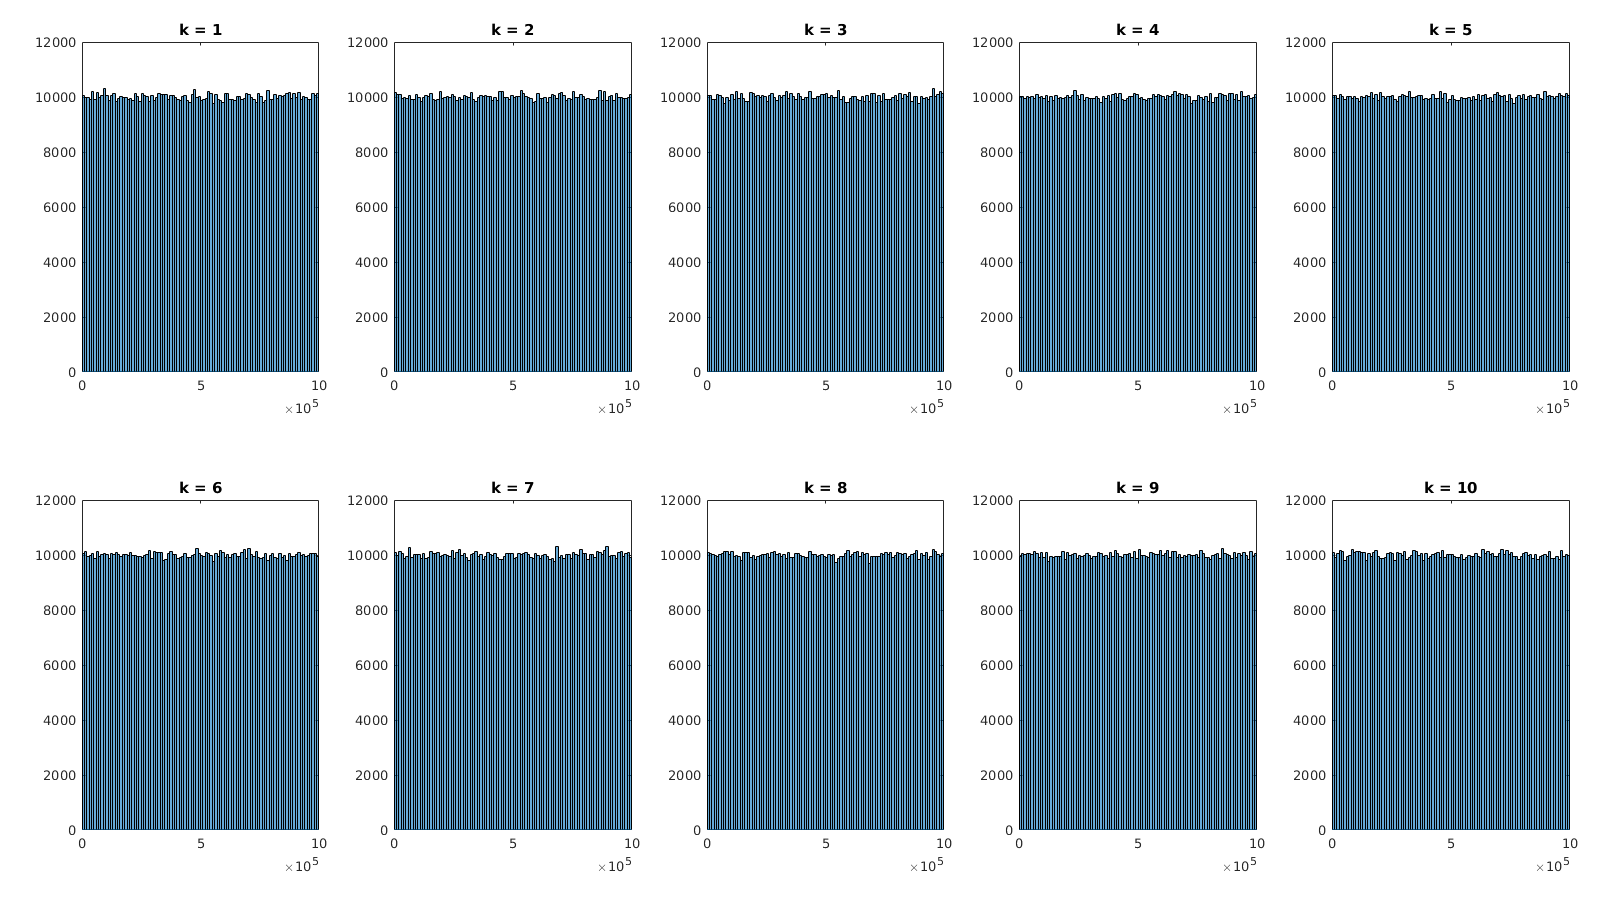
\includegraphics[height=5cm]{img/test_HashFunction_distribution}}
\caption{Resultados das distribuições das \texttt{k} funções de \textit{hashing}}
\label{fig:hashdist}
\end{figure}

\subsection{Correlação das funções de \textit{hashing}}
\label{subsec.hashcorr}

Para que se possam ser utilizar as várias funções de \textit{hashing} eficientemente (neste caso isso significa sem aumento da taxa de falsos positivos), é necessário que estas sejam descorrelacionadas (i.e., que o coeficiente de correlação respetivo seja 0). No entanto, neste trabalho considerar-se-ão valores de coeficiente de correlação inferiores a 0.01 como admissíveis (é muito difícil que estes valores sejam iguais a zero, e portanto aceita-se esta ligeira variação).

Este teste encontra-se no ficheiro \textit{test\_hashFunction\_correlation.m} e, tal como noutros testes, gerar-se-á um \textit{set} de \textit{strings} aleatórias e os respetivos valores de \textit{hashing} para diferentes valores de $k$, a variar entre 1 e 100. No teste, foi criada uma matriz de dimensões $k$ por \texttt{numTests} para guardar as \textit{hashes} para os diferentes pares \textit{k - string}. De seguida, calculam-se os coeficientes de correlação das funções duas a duas utilizando os resultados nas linhas da matriz anterior e a função \texttt{corrcoef} (calcula o coeficiente de correlação entre dois conjuntos, neste caso, duas linhas representativas de dois valores de $k$ distintos).

Por fim, é gerado um gráfico recorrendo à função \texttt{surf} que premite ilustrar os valores de correlação resultantes. Verifica-se que para diferentes valroes de $k$ num par (i.e., comparando $k$s diferentes) os valores se situam geralmente bastante abaixo do erro assumido, havendo alguns picos onde efetivamente o coeficiente de correlação se aproxima deste erro. Conluí-se assim que as funções escolhidas são ``suficientemente'' descorrelacionadas, tal como se pretendia.

\begin{figure}[ht]	
\center
\fbox{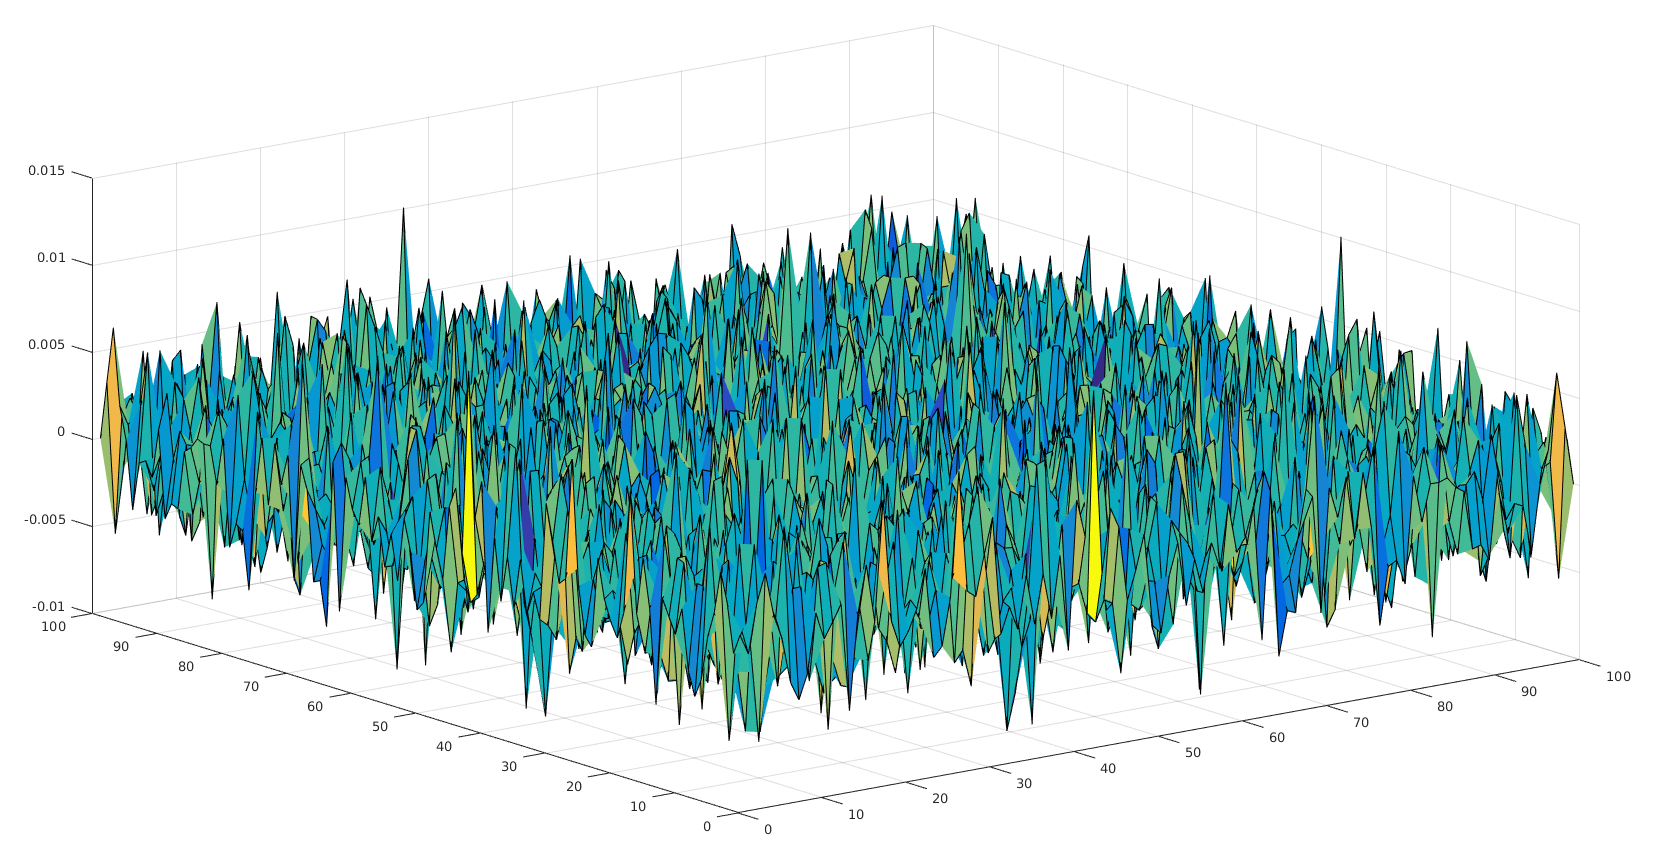
\includegraphics[height=5cm]{img/test_HashFunction_decorrelation}}
\caption{Resultados do teste de correlação de \texttt{k} funções de \textit{hashing}}
\label{fig:hashcorr}
\end{figure}

\subsection{Independência das funções de \textit{hashing}}
\label{subsec.hashindep}

Para além do teste de correlação, foi também efetuado um teste de independência das funções de \textit{hashing} (\textit{test\_hashFunction\_independence.m}), adaptado da implementação do professor António Teixeira. A independência implica descorrelação, e com isto, pode-se provar com qualquer um dos testes que as funções são descorrelacionadas. O objetivo é provar que cada par de colunas é independente entre si.

Primeiramente, é criado um \textit{set} de cem mil \textit{strings} aleatórias e, seguidamente, outra matriz dos respetivos \textit{hash codes} com \texttt{k} (neste teste, \texttt{k = 10}) diferentes \textit{seeds}, utilizando a família de funções \textit{FarmHash}, de tamanho \texttt{k} (número de funções de \textit{hashing} que se pretende aplicar) por \texttt{N} (número de testes que se pretendem executar). De seguida, é gerado um vetor de 10 elementos linearmente espaçados (\texttt{x}) entre 0 e \texttt{N}, e, para cada par de colunas, é criada uma matriz (\texttt{pmf}) de dimensão \texttt{length(x) - 1 / length(x) - 1}. Depois, guarda-se em cada elemento da matriz o número de elementos das colunas de \textit{hash codes} que se situam num mesmo intervalo (esse intervalo é definido pelo vetor \texttt{x} já criado).

Por fim, é calculada a matriz de probabilidade conjunta de duas colunas (\textit{PMF - Probability Mass Function}), e, a partir da mesma, são calculados os vetores de probabilidade individuais de cada uma das colunas. Finalmente, é calculado o resultado da multiplicação destes dois últimos vetores (dois acontecimentos A e B são independentes se $P(A\&B) = P(A) * P(B)$), e compara-se com a matriz de probabilidade conjunta.

\begin{figure}[ht]	
\center
\fbox{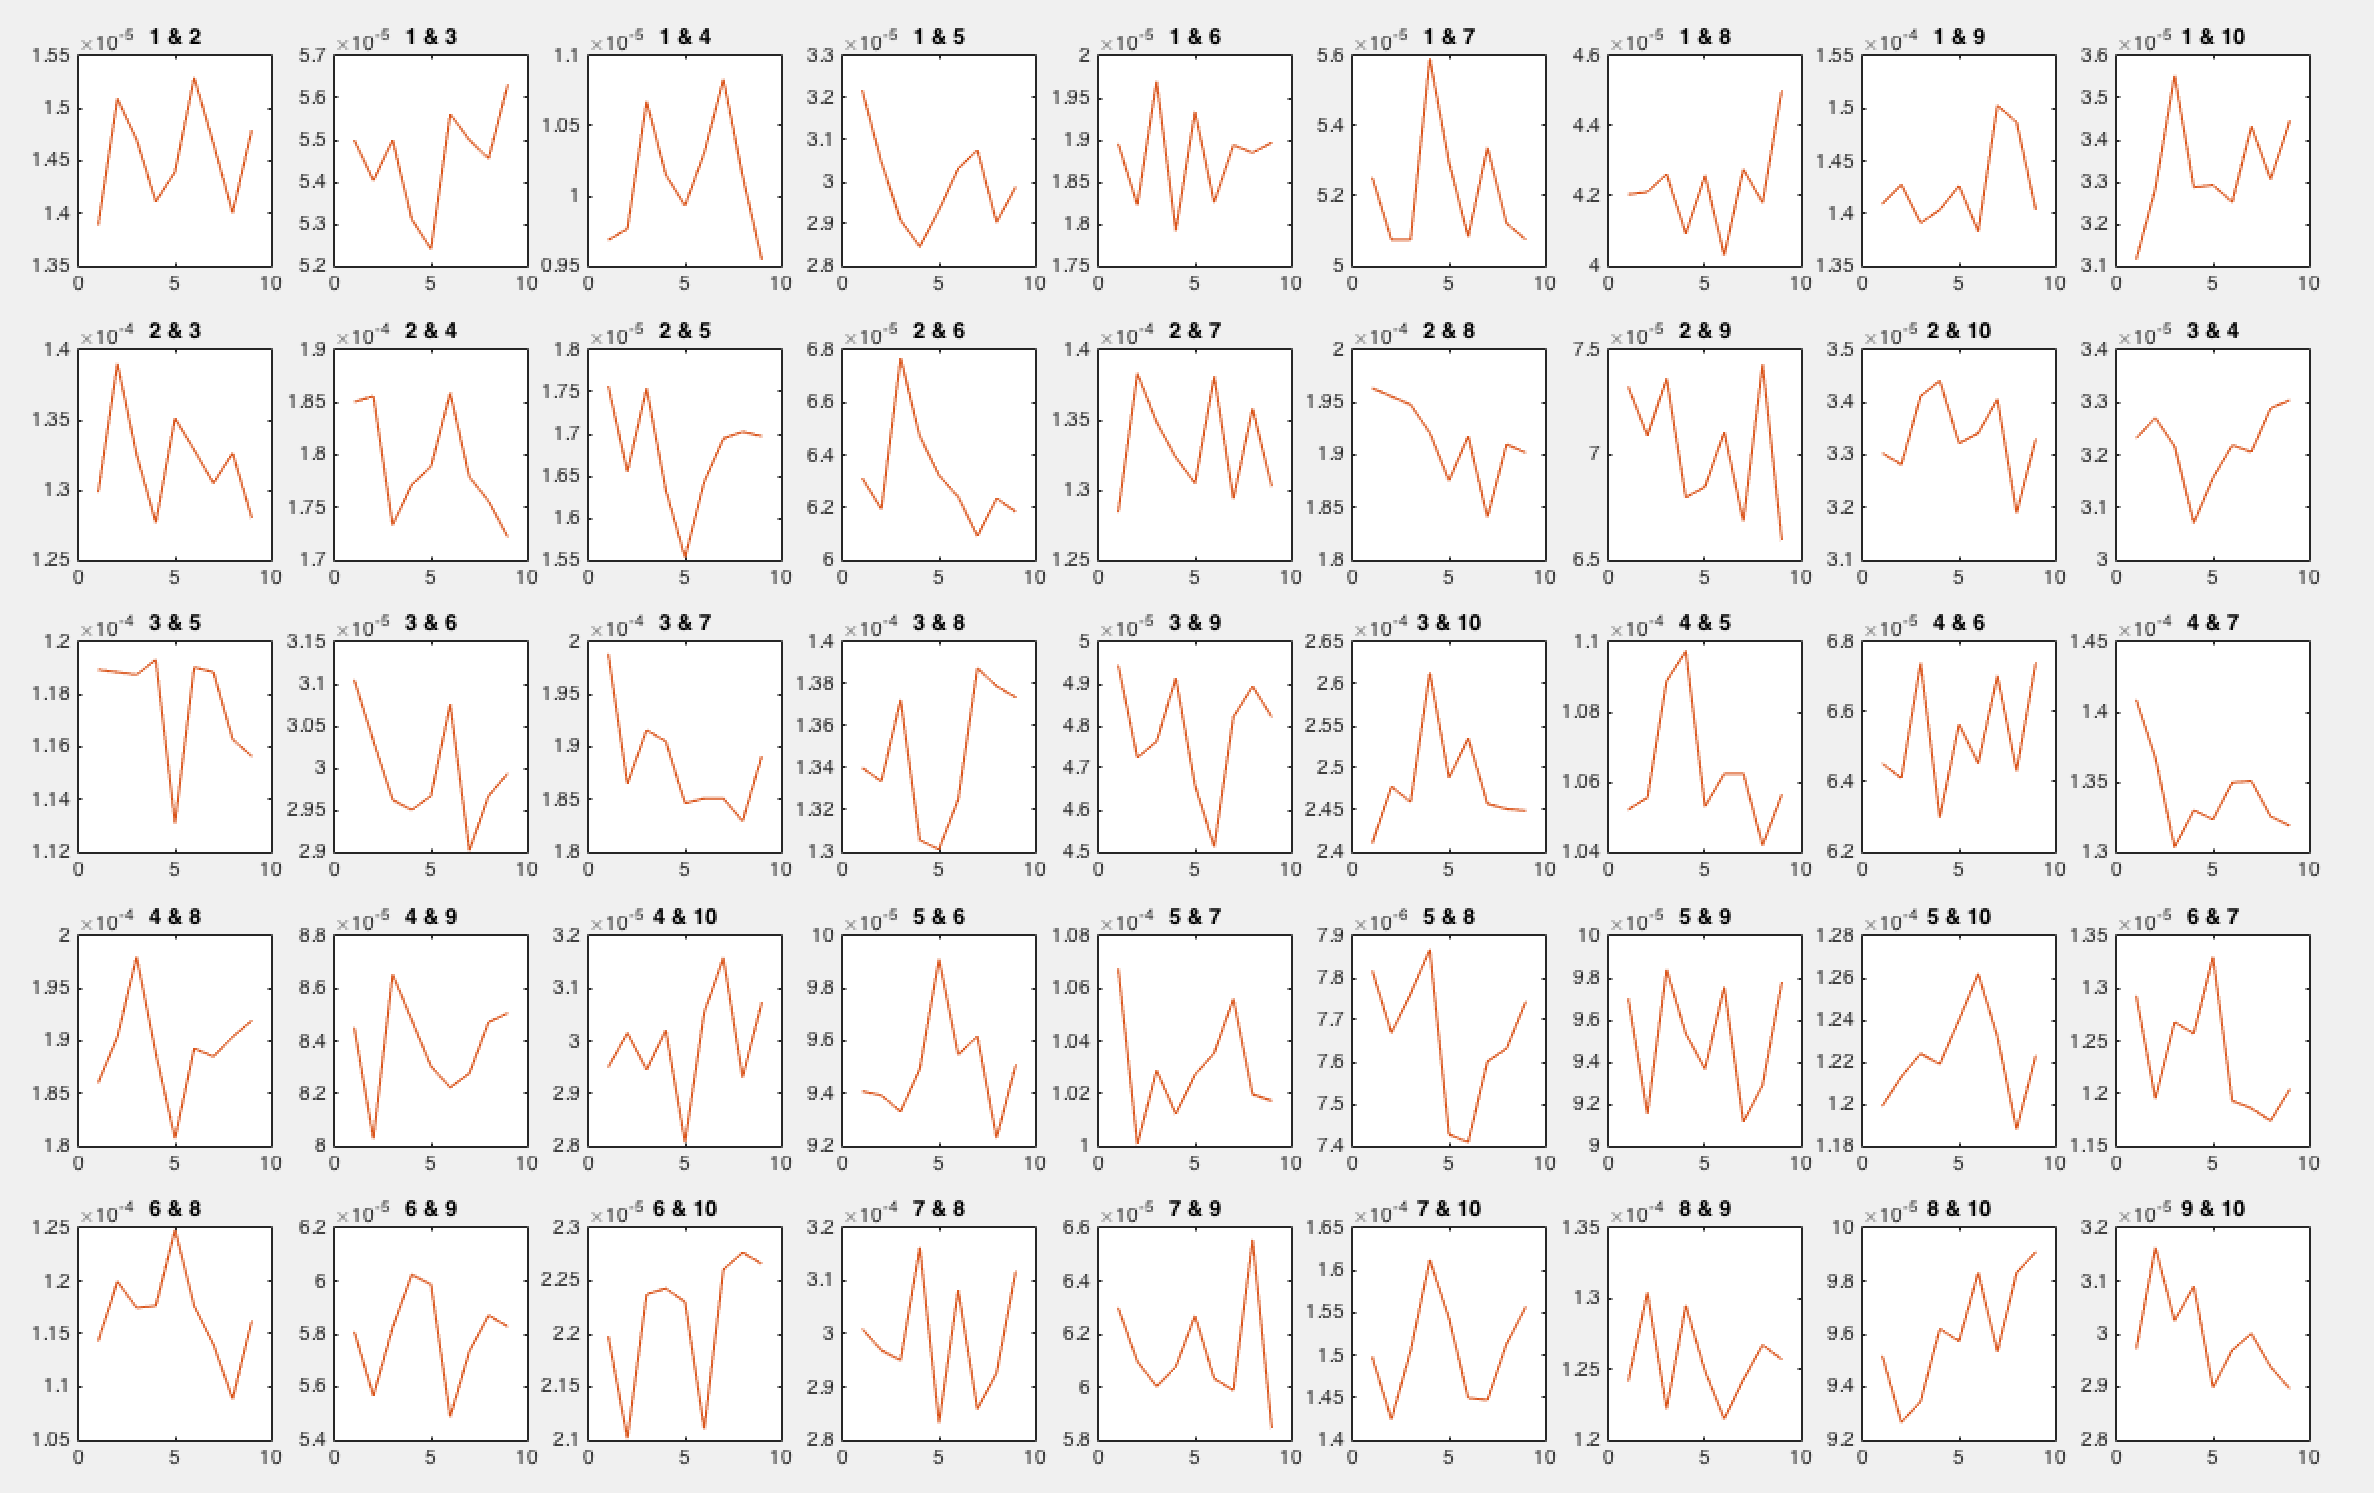
\includegraphics[height=7cm]{img/test_hashFunction_independence}}
\caption{Resultados do teste de independência de \texttt{k} funções de \textit{hashing}}
\label{fig:hashindep}
\end{figure}

Como os valores da variação de resultados são mínimos (como se observa na \autoref{fig:hashindep} todos os valores rondam os $10^-4$), podemos considerar que a família de funções é independente, o que nos leva a concluir que são descorrelacionadas.

\subsection{Número ideal de funções de \textit{hashing}}
\label{subsec.optimalk}

O programa de teste para o valor de \texttt{k} ideal encontra-se com o nome \textit{test\_optimalK.m}.

Começa-se por criar uma instância da classe de \textit{Bloom-filter} anteriormente desenvolvida (com o campo \texttt{debug} inicializado a 1, para que se possam utilizar as funções de alteração de valores) e gerar dois conjuntos (um dos quais será adicionado ao filtro, outro não) distintos de cem mil (valor que pode ser alterado) \textit{strings} (como poderá haver \textit{strings} iguais nos \textit{sets}, o tamanho será sempre ligeiramente inferior ao definido anteriormente). De seguida, define-se o tamanho do vetor de \textit{bits} do filtro como oito vezes maior do que o tamanho dos conjuntos de \textit{strings} gerados.

Por fim, itera-se sobre um vetor de \texttt{k} que se definira anteriormente (neste caso, é um vetor com valores de 1 a 15) e, cada ciclo, define-se um \texttt{k} no \textit{Bloom-filter}, adiciona-se os elementos do vetor incialmente escolhido como aquele que se iria adicionar ao filtro e verifica-se se algum dos elementos do outro conjunto de \textit{strings} pertence ou não ao filtro. Caso pertença, é incrementado um contador, para, no final do ciclo, ser calculada a probabilidade de falsos positivos.

\begin{figure}[ht]	
\center
\fbox{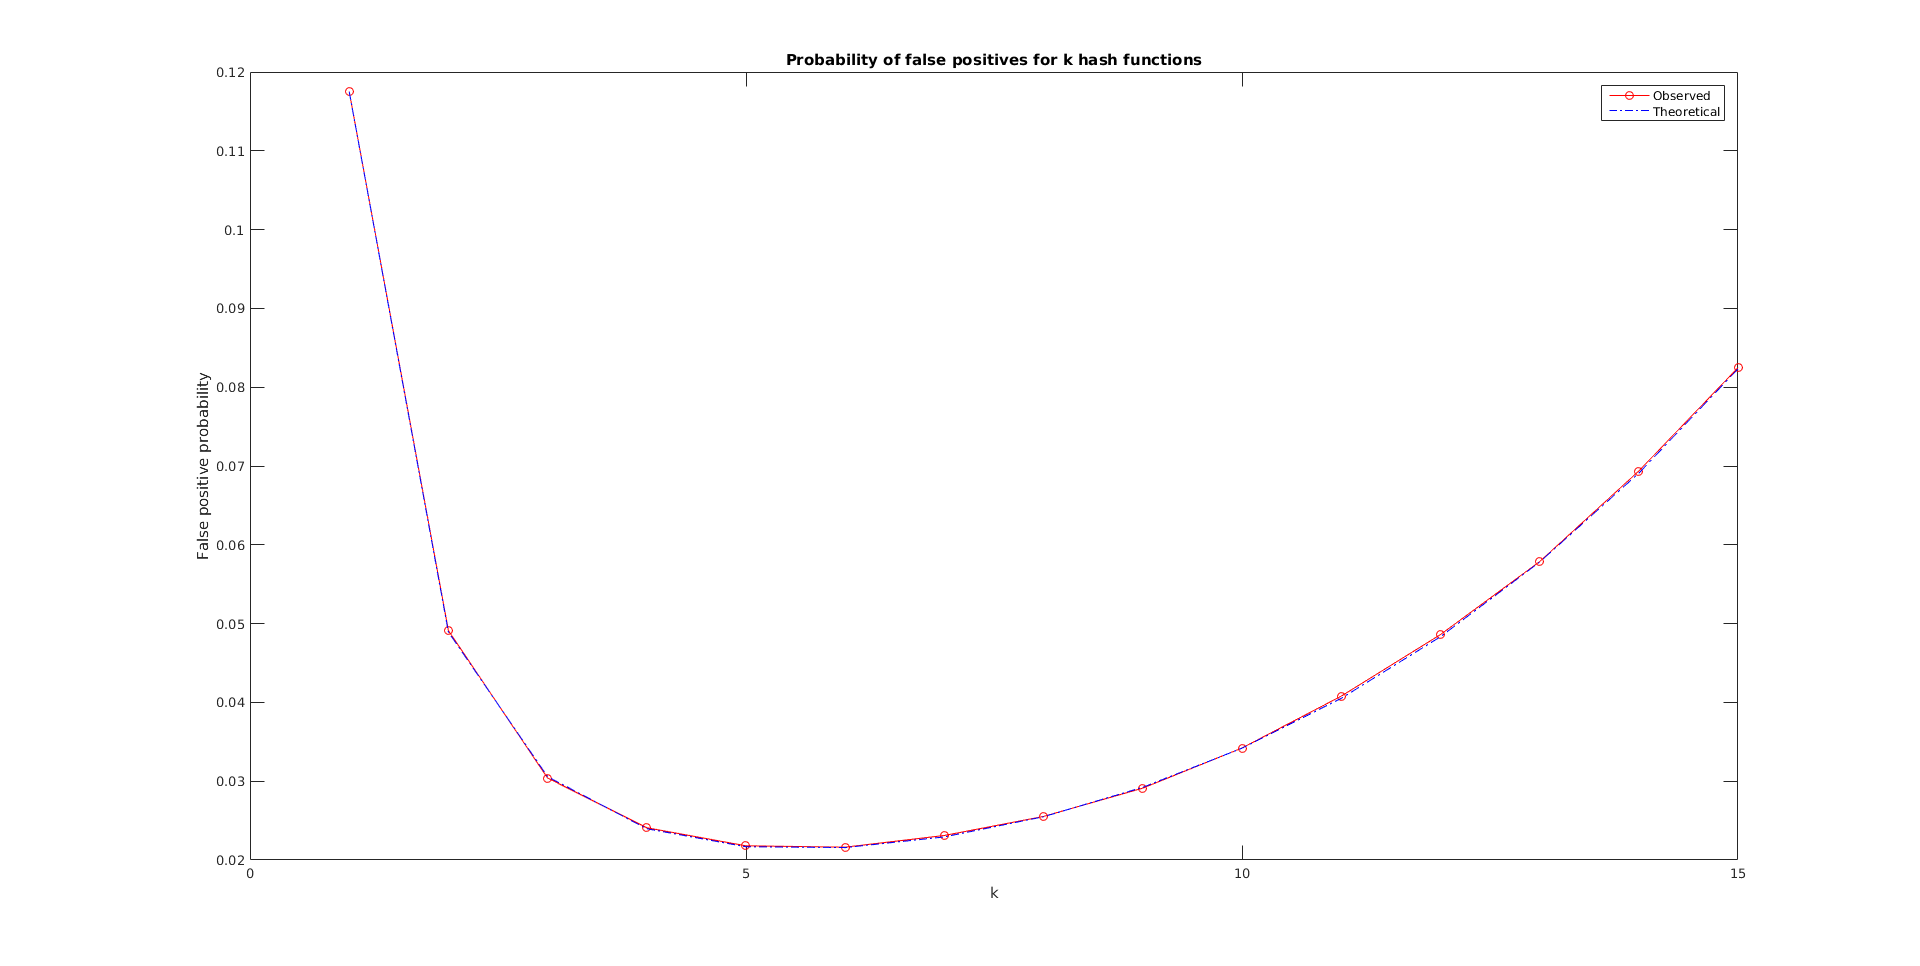
\includegraphics[height=5cm]{img/test_OptimalK}}
\caption{Resultados do teste do valor ideal de funções de \textit{hashing} (\texttt{k})}
\label{fig:optimalk}
\end{figure}

De acordo com o gráfico da \autoref{fig:optimalk}, usando a fórmula 

$$ p =  \left(1 - e^{-\frac{km}{n}}\right)^k $$

para determinar a probabilidade de falsos positivos (teórica) para diferentes valores de \texttt{k} e usando os valores do teste acima, verificamos que as diferenças entre o valor teórico e observado são mínimas (o que significa que a função de \textit{hashing} devolve excelentes resultados, mas isso será abordado mais abaixo), e que o valor ideal é 6, para a função de \textit{hashing} em questão. Para uma função diferente, os valores poderão diferir.

\subsection{Número ideal do vetor de \textit{bits}}
\label{subsec.optimaln}

O módulo para o teste do valor ideal do tamanho do vetor \texttt{n} encontra-se no ficheiro \textit{test\_optimalN.m}.

Tal como no teste do \autoref{subsec.optimalk}, também são criados dois conjuntos de \texttt{strings} aleatórias com o mesmo propósito, um para ser adicionado ao filtro e o outro não. É também criado um vetor com diferentes valores de \texttt{n}, que vão desde o tamanho dos conjuntos de \textit{strings} até 10 vezes esse valor, com uma diferença de metade do mesmo valor entre cada.

De seguida, itera-se sobre os valores deste último vetor de valores e vai-se criando uma instância de um \textit{Bloom-filter} com os valores de \texttt{n} (\texttt{arraySize}) e \texttt{k} (depende do tamanho do vetor) a cada passagem. Adiciona-se um dos conjuntos de \textit{strings}, verifica-se a existência dos elementos do outro que não foi adicionado e, por fim, calcula-se a probabilidade de falsos positivos, tal como no teste anterior.

\begin{figure}[ht]	
\center
\fbox{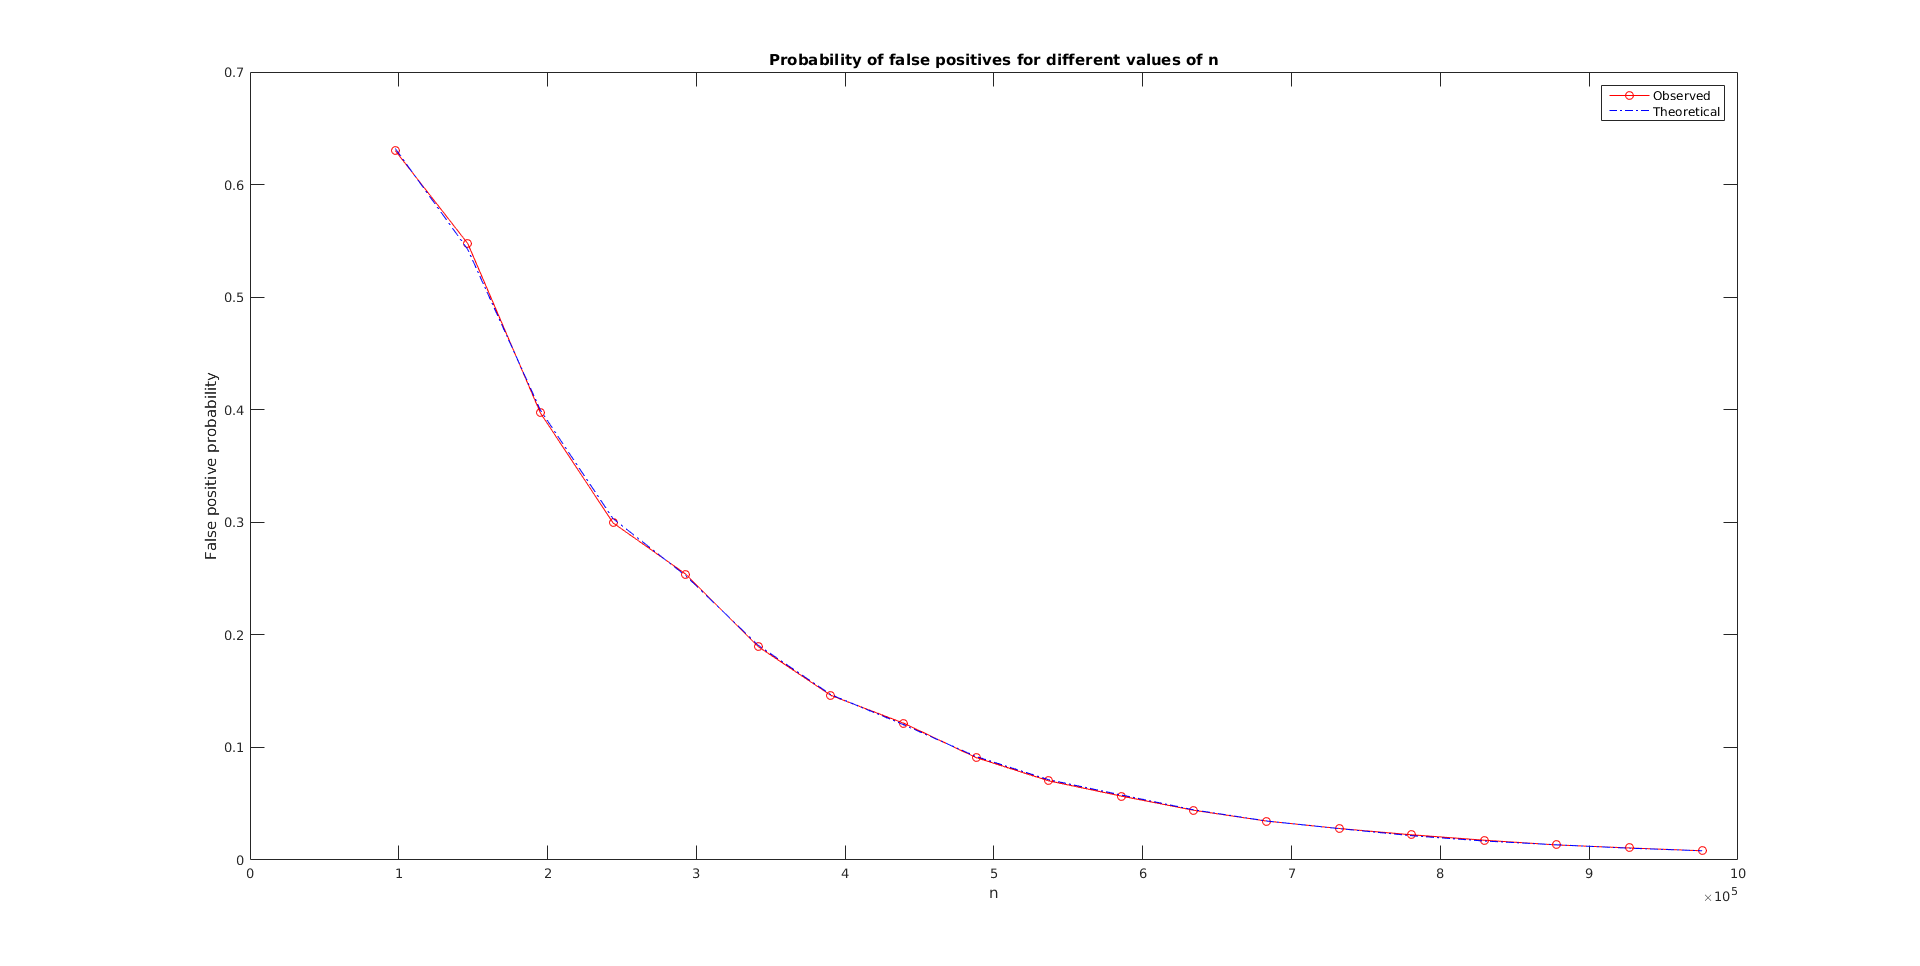
\includegraphics[height=5cm]{img/test_OptimalN_img}}
\caption{Resultados o teste do tamanho ideal do vetor de \textit{bits} (\texttt{arraySize} / \texttt{n})}
\label{fig:optimalnimg}
\end{figure}

Como se verifica no gráfico da \autoref{fig:optimalnimg}, à medida que o tamanho do \textit{array} aumenta, a probabilidade de falsos positivos diminui, isto é, são inversamente proporcionais.

Os valores ideias são os presentes na \autoref{fig:optimalntext}

\begin{figure}[ht]	
\center
\fbox{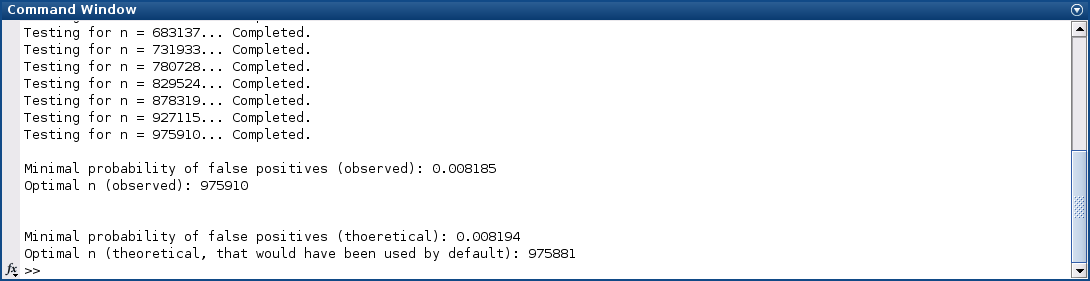
\includegraphics[height=5cm]{img/test_OptimalN_txt}}
\caption{Resultados ideias do tamanho ideal do vetor de \textit{bits} (\texttt{arraySize} / \texttt{n})}
\label{fig:optimalntext}
\end{figure}

\subsection{Testes práticos do \textit{Bloom-filter}}
\label{subsec.testebloom}

Foram desenvolvidos dois módulos semelhantes para um teste mais direcionado ao uso real de um \textit{Bloom-filter}. Estão em dois ficheiros distintos, \textit{test\_big\_BloomFilter.m} e \textit{test\_small\_BloomFilter.m}.

O primeiro segue o modelo dos testes anteriores, em que se gera dois \textit{sets} de um certo tamanho (neste caso, cem mil elementos) de \textit{strings} aleatórias, cria-se uma instância de um \textit{Bloom-filter} com uma probabilidade de falsos positivos de 0.0001\%, adiciona-se um dos conjuntos ao filtro e verifica-se a existência de falsos positivos. Por fim, compara-se o resultado observado da probabilidade de falsos positivos com a que se definiu aquando a criação do filtro. O objetivo é que os resultados sejam o mais próximos possíveis, algo que se conseguiu atingir em ambos os testes.

No segundo teste (\textit{small}), contrariamente ao primeiro em que se geram os conjuntos, definem-se conjuntos muito pequenos inicialmente e, depois, executa-se o mesmo processo que o anterior.

\begin{figure}[ht]	
\center
\fbox{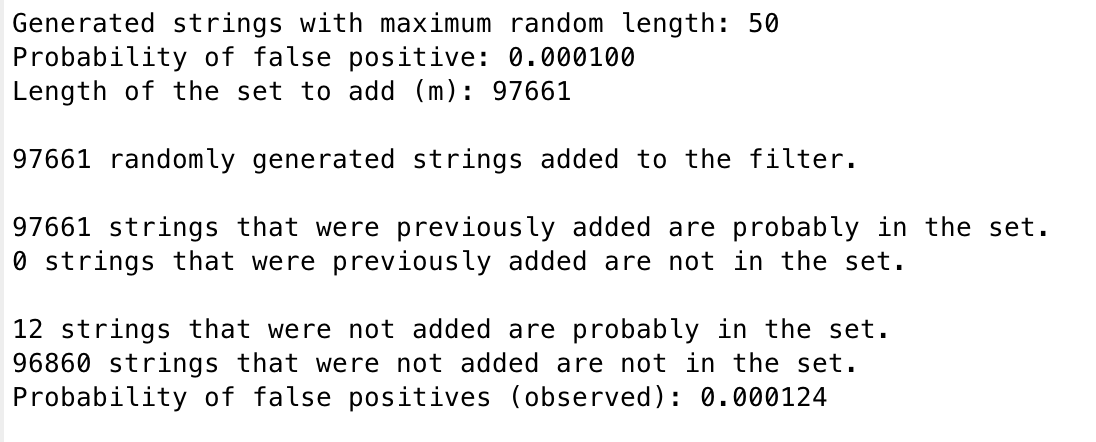
\includegraphics[height=5cm]{img/test_big_BloomFilter}}
\caption{Resultados da execução de \textit{test\_big\_BloomFilter.m}}
\label{fig:testbigbloom}
\end{figure}


\chapter{Locality-Sensitive Hashing}
\label{chap.lsh}

O \textit{Locality-Sensitive Hashing} é particularmente útil quando se têm grandes conjuntos de documentos e se pretende achar semelhantes entre si, como, por exemplo, achar notícias semelhantes em diversos \textit{websites}. No entanto, pequenos trechos dos documentos podem aparecer noutros não necessarimente na mesma ordem. Para além do mais, se tivermos \textit{sets} na ordem dos milhões e milhares de milhão, são tantas as comparações que são necessárias fazer que excedem a memória disponível.

Portanto, para podermos comparar documentos, são necessários 3 passos:

\begin{description}
\item[Shingling]
Converter documentos para conjuntos.
\item[Min-Hashing]
Converter grandes conjuntos para pequenas assinaturas (por norma, de inteiros), preservando a similariedade.
\item[Locality-Sensitive Hashing]
Forcar-se apenas nos pares de assinaturas que possivelmente pertençam a documentos semelhantes e, mais tarde, testar realmente a sua similariedade.
\end{description}

O módulo de \textit{LSH} está no ficheiro \textit{LSH.m} e dispõe dos seguintes métodos:

\begin{description}
\item[shingleWords]
Aceita um \textit{cell array} com o conteúdo de um documento e devolve \textit{shingles} relativos ao mesmo.
\item[signature]
Converte um vetor de \textit{shingles} num vetor de assinaturas, através do processo de \textit{min-hashing}.
\item[candidates]
Devolve a lista de documentos candidatos a serem semelhantes a outros, consoante a matrix de assinaturas e o \textit{threshold} passados como argumentos.
\item[candidates\_to]
Executa o mesmo processo que a função \texttt{candidates}, no entanto, em vez de aceitar apenas uma matriz de assinaturas, aceita também a assinatura de um documento, o qual pretendemos comparar com os restantes.
\item[similars]
Verifica quais são os documentos realmente semelhantes e a sua Similariedade de Jaccard, consoante a matriz de candidatos, assinaturas e o \textit{threshold} passados como argumentos.
\item[similiars\_to]
Tem a mesma função que \texttt{similars}, no entanto, aplica-se ao caso em que pretendemos comparar um documento com os restantes.
\end{description}

O único construtor do módulo aceita apenas um argumento, que é o erro esperado (\texttt{expectedError}). Este erro será utilizado para calcular o número \texttt{k} de \textit{hash functions} necessárias, que é também o único atributo que o módulo possui, segundo a fórmula:

$$ k = 1 / expectedError^2 $$

\subsection{Shingling}
\label{subsec.shingling}

Uma \textit{k-shingle} de um documento é uma sequência de k \textit{tokens} (palavras, caracteres, etc.) que aparecem no documento. Documentos que tenham muitas \textit{shingles} em comum, possuem texto parecido, mesmo que o mesmo não apareça na mesma ordem.

A similariedade entre dois documentos ($D1, D2$) pode ser calculada através da Similariedade de Jaccard:

$$ sim(D1, D2) = \frac{|C1\cap C2|}{|C1\cup C2|} $$

sendo $C1$ e $C2$ os conjuntos de \textit{shingles} de $D1$ e $D2$, respetivamente.

A Distância de Jaccard, por outro lado, pode ser dada por:

$$ d(D1, D2) = 1 - sim(D1, D2) $$

Para gerar um \textit{set} de \textit{shingles} é utilizada a função \texttt{shingleWords}, que recebe como argumento um \textit{cell array}, neste caso, de \textit{strings} (considere-se o mesmo \texttt{Doc}). Para gerar esse conjunto, é necessário selecionar quais as sequências de palavras mais importantes de \texttt{Doc}. Para tal, é necessária a criação de um \textit{set} de \textit{stop words}, logo, foram guardadas num \textit{cell array} \texttt{stop\_words} as cem palavras mais comuns da língua inglesa. Quando o programa encontra uma \textit{stop word}, ele guarda a sequência \textit{stop\_word next\_word1 next\_word2} num outro \textit{cell array}, que será o retorno da função.

\subsection{Min-Hashing}
\label{subsec.minhash}

Para contornar as demoras que as comparações de excertos de textos provocariam, os \textit{shingles} são convertidos em assinaturas de inteiros, no entanto, a sua similariedade deve ser conservada.

Para a criação das respetivas assinaturas é usada a função \texttt{signature}; começa-se por se criar um vetor em que o seu valor inicial é o valor máximo do tipo \textit{double} (auxilia no cálculo dos valores mínimos) e, de seguida, para cada valor de \texttt{k} (número de \textit{hash functions}), é gerado um vetor das assinaturas do \textit{cell array} de \textit{shingles} que é passado como argumento, dos quais é extraído o valor mínimo e guardado no \textit{array} mais tarde devolvido pela função.

\subsection{Locality-Sensitive Hashing}
\label{subsec.lsh}

Por fim, depois de gerados os vetores de assinaturas dos documentos, basta compará-los e ver quais aqueles que mais se assemelham.

Primeiramente, começa-se por definir uma lista de candidatos possíveis (onde é provável a ocorrência de falsos positivos), para, por fim, verificar quais são mesmo os documentos que são realmente semelhantes (segundo um coeficiente de Similariedade - \textit{threshold}).

A função \texttt{candidates}, definida no módulo \texttt{LSH}, serve para definir a lista de candidatos possíveis. Consideremos a matriz de assinaturas \textit{M}, em que cada coluna corresponde à assinatura de um documento, isto é, o resultante do processo de \textit{min-hashing} dos \textit{shingles} obtidos.

% Explicar o processo de encontrar r rows e b bands

Cria-se também um \textit{cell array} onde serão armazenados os pares candidatos a serem semelhantes, numa estrutura em que a linha \textit{i} corresponde ao documento \textit{i} e em que cada coluna corresponde ao índice \textit{j} de um documento possível candidato semelhante ao documento \textit{i}.

De seguida, itera-se sobre cada uma das bandas que se extraem da matriz de assinaturas e compara-se com todas as outras bandas existentes (verica-se se a soma do número de assinaturas que as bandas têm em comum é igual ao número de \textit{rows}).

Por fim, a função \texttt{similars} trata de finalizar o processo e devolver os documentos que são realmente semelhantes e o seu coeficiente de similariedade.

Itera-se sobre a matriz de candidatos e compara-se, uma a uma, se a Similariedade de Jaccard entre as assinaturas é maior que o \textit{threshold} definido (usando a função \texttt{intersect}, que devolve os elementos em comum entre dois conjuntos). Se a condição se verifica, adiciona-se ao vetor de retorno os índices na matriz de assinaturas dos documentos em questão e o valor da sua similariedade.

\subsection{Testes}
\label{subsec.lshtests}
Para os testes deste módulo, foram adaptados os \textit{scripts} do Guião Prático-Laboratorial 07 da disciplina, mas, para além de ser usado o \textit{dataset} de cem mil utilizadores da MovieLens, foi também utilizado o que contém um milhão de utilizadores.

A única diferença entre os testes é apenas o \textit{dataset} utilizado, pois o processo tem de obrigatoriamente ser o mesmo, apenas se muda o tamanho do conjunto de dados.

Inicia-se o teste obtendo um vetor com todos os utilizadores a partir do \textit{dataset}. De seguida, para cada utilizador, constrói-se o conjunto de \textit{shingles} (neste caso, não é usada a função \texttt{shingleWords} do módulo \texttt{LSH}, visto que não é documento de texto, mas sim um vetor de de índices de filmes que cada utilizador avaliou) e respetivas assinaturas, usando a função \texttt{signature}. 

Primeiro, vai ser calculada a Similariedade de Jaccard esperada (teórica), simplesmente iterando sobre o conjunto de assinaturas e, usando a fórmula 

$$ sim(D1, D2) = \frac{|C1\cap C2|}{|C1\cup C2|} $$

e as funções de Matlab \texttt{intersection} (devolve os elementos que dois conjuntos têm em comum) e \texttt{union} (devolve a união de dois conjuntos). Por fim, verifica-se, quais destes valores estão a acima do \textit{threshold} assumido (nestes teste, assumiu-se 0.6). Os resultados mostram que existem apenas 3 documentos com uma similariedade acima dos 0.6, como se verifica na \autoref{fig:test100ke}.

\begin{figure}[ht]	
\center
\fbox{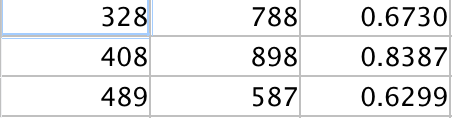
\includegraphics[height=2cm]{img/test_LSH_100k_Exp}}
\caption{Resultados (valores esperados) do teste com 100 mil utilizadores}
\label{fig:test100ke}
\end{figure}

Finalmente, para calcular a Similariedade de Jaccard observada (experimental), gera-se a lista de candidatos usando a função \texttt{candidates} do módulo \texttt{LSH} e a matriz com os documentos similares usando a função \texttt{similars}, também do mesmo módulo.

A \autoref{fig:test100ko} mostra que os resultados de ambos os testes foram os mesmos, havendo apenas uma pequeníssima variação dos valores de similariedade (à volta de 0.2).

\begin{figure}[ht]	
\center
\fbox{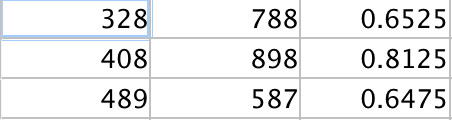
\includegraphics[height=2cm]{img/test_LSH_100k_Obs}}
\caption{Resultados (valores observados) do teste com 100 mil utilizadores}
\label{fig:test100ko}
\end{figure}

% Falta teste com dataset de 1m

\chapter{SPAM Filter}
\label{chap.spamfilter}

A filtragem de \textit{email}  é uma maneira de o organizar segundo um certo critério; é largamente utilizado para filtrar \textit{spam} e vírus eletrónico a caixa de entrada de uma conta de email.

Uma maneira de filtrar o \textit{spam} de uma caixa de entrada é comparar o conteúdo de \textit{emails} previamente consideramos como tal e ver se são semelhantes. Outro método é verificar se o endereço de \textit{email} da nova mensagem já enviara algum mail de \textit{spam} anteriormente.

Um \textit{Bloom-filter} e o \textit{Locality-Sensitive Hashing} são particularmente úteis nesta matéria.

O \textit{Bloom-filter} servirá como armazenamento de endereços de \textit{email} que previamente tinham enviado lixo, enquanto que o \textit{Locality-Sensitive Hashing} servirá para comparar o conteúdo de novas mensagens com antigas mensagens de \textit{spam}.

Primeiro é necessário que o programa "aprenda" que \texit{emails} deve filtrar. Para tal, foi utilizado dois \textit{datasets}, CSMining e Enron, em que se insere uma série de mensagens de \textit{spam} e \texit{ham} (\texit{non-spam}) devidamente identificados. A função \texttt{create\_generic} aceita um diretório onde vai procurar pelos ficheiros da extensão que também lhe é passada como argumento, para guardar num ficheiro (o caminho também é passado como argumento) o \textit{Bloom-filter} com os endereços de email que enviaram \textit{spam}, as assinaturas do conteúdo dos mesmos e o módulo de \textit{LSH} usado (para salvaguardar o número de funções de \textit{hashing} utilizadas).

Por outro lado, a função \texttt{test\_generic} testa o filtro de \textit{spam} com base no ficheiro previamente guardado. Os dados desse mesmo ficheiro são carregados para o programa e todos os \textit{emails} contidos na pasta que é passada como argumento da função são analisados.

\chapter{Conclusões}
\label{chap.conclusões}

\maketitle
\nocite{*}
\printbibliography[title={Referências}]

\end{document}
